%%=============================================================================
%% Methodologie
%%=============================================================================

\chapter{\IfLanguageName{dutch}{Methodologie}{Methodology}}
\label{ch:methodologie}

\section{Type onderzoek}
Het onderzoek beschreven in deze tekst is een \textbf{kwantitatief} onderzoek. Voor combinaties van het aantal auto's en het aantal reservaties zullen het service level, de totale gebruiksduur van de auto's en de tijdsduur van de reservaties die niet konden doorgaan vergeleken worden. Vanuit een bedrijfsstandpunt is het interessant om het service level en de gebruiksduur van de auto's maximaliseren voor een gegeven grootte van de vloot. Voor dit onderzoek wordt geopteerd voor een aanpak die zo dicht mogelijk aansluit bij de realiteit binnen het bestek van het onderzoek. In de stand van zaken werd een theoretische aanpak beschreven door middel van wachtrijtheorie. Een belangrijke stap hierbij is het bepalen van de parameter $\Lambda$ van het Poisson-proces dat de aankomst van reservaties modelleerd. Deze $\Lambda$ is echter tijdsafhankelijk en niet hetzelfde voor elke dag van de week of periode van het jaar. In dit onderzoek worden simulaties uitgevoerd uit met een zelf-ontwikkelde simulatietool die historische reservaties van Partago gebruikt. De programmeercode van deze simulatietool is als bijlage opgenomen bij deze scriptie. Deze simulaties simuleren reëel reservatiegedrag van de Partago gemeenschap aangezien het gaat om echte reservaties. Verder in dit hoofdstuk wordt exact beschreven hoe deze simulaties zijn opgebouwd en welke stappen binnen elke simulatie uitgevoerd worden om tot numerieke waarden voor het service level en de gebruiksduur van de auto's te komen. 

\section{Opzet van een simulatie}
\subsection{Doel}
Tijdens de simulatie wordt er een getracht tweemaal een toewijzing te doen van de beschikbare auto's aan de reservaties in de simulatie. Eenmaal zal deze toewijzing gebeuren op een eenvoudige manier (zie verder) en eenmaal zal deze toewijzing gebeuren door het oplossen van het corresponderende Constraint Satisfaction Problem (zie verder en stand van zaken). Voor beide toewijzingen wordt dan het service level, de tijd dat de auto's actief waren en de tijd van reservaties die niet konden doorgaan omdat er geen auto beschikbaar was berekend. Een CSP oplosalgoritme geeft een oplossing voor het probleem, maar niet per se de meest optimale oplossing (zie ook stand van zaken). Daarom werd elke karakteriserende simulatie meermaals uitgevoerd. Hierdoor kan per set van karakteristieke parameters een gemiddelde en standaard afwijking berekent worden. 

\subsection{Karakteristieken}
Eén enkele simulatie wordt gekarakteriseerd door waarden van de volgende grootheden:
\begin{itemize}
	\item \textbf{Aantal reservaties in de simulatie:}
	Het aantal reservaties is een maat voor de drukte op het systeem. Het aantal gebruikers van het systeem zou hier geen goede maat voor zijn, weinig gebruikers kunnen immers ook relatief veel reservaties maken. Veel reservaties betekent een grote drukte op het systeem, weinig reservaties betekent een kleine drukte. Uiteraard kunnen overlappende reservaties niet van dezelfde persoon afkomstig zijn. De reservaties gebruikt in de simulatie zijn bestaande historische reservaties van Partago.
	\item \textbf{Aantal auto's:}
	Tijdens de simulatie zullen er toewijzingen gebeuren van de auto's aan de reservaties. Meer auto's beschikbaar in de fictieve zone zal het service level onmiddellijk doen toenemen. Voor eenzelfde aantal reservaties zullen meer reservaties kunnen doorgaan als er meer auto's beschikbaar zijn. 
	\item \textbf{Aantal weken:}
	Elke simulatie stelt een fictieve reserveringsperiode voor van een aantal weken. Tijdens dit onderzoek wordt deze parameter vastgehouden op \textbf{2 weken}. Tijdens elke simulatie zullen we dus een periode van 2 weken simuleren. 
\end{itemize} 

\subsection{Stappen binnen een simulatie}
Binnen één enkele simulatie worden de volgende stappen ondernomen
\begin{enumerate}
	\item Definiëren van de karakteriserende parameters
	\item Historische Partago reservaties ophalen
	\item Een dataset van reservaties genereren op basis van de historische gegevens voor de gedefinieerde periode
	\item Een eenvoudige toewijzing doen van auto's op de reservaties uit de dataset
	\item Een toewijzing doen van auto's op de reservaties uit de dataset met behulp van een CSP oplosalgoritme 
	
\end{enumerate}
Op elk van deze stappen wordt dieper ingegaan in de komende secties van dit hoofdstuk. 

\section{Definiëren van de karakteriserende parameters}
\subsection{Aantal reservaties}
Om een idee te krijgen hoeveel reservaties er zich in een dataset moeten bevinden werden de historische reservaties van Partago geanalyseerd om een inzicht te krijgen in de huidige drukte op het systeem. Het gemiddelde aantal reservaties per week per auto werd berekend voor de periode van 1 januari 2019 tot en met 30 juni 2019. Voor het Partago systeem waren er voor deze periode gemiddeld 2,9117 reservaties per week per auto die zijn doorgegaan. Dit getal houdt enkel rekening met reservaties die effectief zijn doorgegaan en die gedaan zijn door echte gebruikers (dus bijvoorbeeld niet door het onderhoudsteam). Hoeveel reservaties niet konden doorgaan weet het Partago systeem niet. Uit dit gemiddelde kan wel het vermoeden afgeleidt worden dat het Partago systeem momenteel een niet druk systeem is, de vloot relatief onbezet en nagenoeg een service level van 100\% bereikt zal worden. Het aantal reservaties is discreet, het bovenvermelde gemiddelde wordt afgerond tot 3. Voor de uit te voeren simulaties zal de drukte op het systeem opgedreven worden: maal factor 3, factor 5 en factor 10. Het aantal reservaties zal dus variëren van 9 reservaties per week per auto tot 30 reservaties per week per auto. Er wordt gekozen om te starten met een factor 3 aangezien voor factor 2 er gemiddeld 6 reservaties per week per auto zijn. Dit is nog steeds, gemiddeld gezien, nog niet 1 reservatie per dag waardoor een toewijzingsalgoritme niet aan de orde is.
\subsection{Aantal auto's}
Het aantal auto's in een simulatie is afhankelijk van het gekozen aantal reservaties en de drukte die hier mee overeenstemt. Zo is het niet interessant om op een niet druk systeem een simulatie uit te voeren met 50 auto's. Dit is geen reële situatie. Binnen het huidige systeem van Partago telt een zone 1, 2 of 3 auto's. Er wordt dus in de eerste plaats gekozen voor een relatief klein aantal auto's tijdens de simulaties aangezien dit het dichtste aansluit bij hoe Partago momenteel georganiseerd is. Naarmate het aantal auto's stijgt, hoe complexer het probleem. Bij meer complexere problemen wordt een grotere winstmarge verwacht van de toewijzing met behulp van CSP ten opzichte van de eenvoudige toewijzing. Er wordt gekozen om voor elke druktegraad een simulatie uit te voeren worden met 3 en 5 auto's. Voor de drukste systemen wordt ook een simulatie uitgevoerd met 10 auto's.
\subsection{Aantal weken}
Deze parameter vastgehouden worden op 4 weken. Deze keuze is arbitrair. De simulaties over een langere periode laten lopen zou de rekentijd aanzienlijk verhogen en weinig meerwaarde bieden. Zoals eerder vermeld wordt een simulatie met een set van parameters meermaals uitgevoerd zodat de resultaten uitgemiddeld worden. Het lijkt misschien logisch om deze parameter groter te nemen, maar over langere periodes spelen seizoensgebonden factoren, zoals schoolvakanties, mee een grote rol en deze worden niet opgenomen in dit onderzoek.
\subsection{Uit te voeren simulaties}
De simulaties die uitgevoerd zullen worden worden weergegeven in volgende tabel:
\begin{center}
	\begin{tabular}{ | l | l | l | p{3cm} |}
		\hline
		Aantal reservaties & Aantal auto's & Druktegraad & Aantal weken \\ \hline
		108 & 3 & 9 reservaties/week/auto & 4 \\ \hline
		180 & 5 & 9 reservaties/week/auto & 4 \\ \hline
		180 & 3 & 15 reservaties/week/auto & 4 \\ \hline
		300 & 5 & 15 reservaties/week/auto & 4 \\ \hline
		360 & 3 & 30 reservaties/week/auto & 4 \\ \hline
		600 & 5 & 30 reservaties/week/auto & 4 \\ \hline
		1200 & 10 & 30 reservaties/week/auto & 4 \\ \hline
	\end{tabular}
\end{center} 

\section{Partago reservaties ophalen}
De dataset van reservaties die gegenereerd wordt is gebaseerd op bestaande reservaties uit het verleden gedaan op het systeem van Partago. Dit geeft als voordeel dat de dataset een reëel karakter zal vertonen en dus dicht aansluit op werkelijk reserveringsgedrag. Voor dit onderzoek worden historische gegevens van Partago van 1 januari 2019 tot en met 30 juni 2019 gebruikt. Voor filtering zijn dit 7533 reservaties die gebruikt kunnen worden om datasets uit te generen. Dit aantal wordt wel nog opgekuist vooraleer de dataset gegenereerd wordt: reservaties niet uitgevoerd door Partago-coöperanten (bijvoorbeeld door het onderhoudsteam), reservaties korter dan 5 minuten, reservaties langer dan 24uur en geannuleerde reservaties worden verwijderd.

\section{Dataset van reservaties genereren}
Uit de gefilterde lijst van Partago reservaties zal een dataset van reservaties gegenereerd worden voor een periode van het gedefinieerde aantal weken. In dit onderzoek zal elke dataset dus bestaan uit reservaties voor 4 weken. De parameter ``aantal reservaties`` zal bepalen hoeveel reservaties zich in de dataset bevinden. Dit aantal wordt willekeurig geselecteerd uit de historische Partago reservaties en gemapt op een willekeurige week in de dataset (week1, week2, week3 of week4), maar met behoudt van de dag van de week. Reservatiegedrag op een dinsdag is mogelijks niet hetzelfde als reservatiegedrag op een zaterdag. Deze informatie mag dus niet verloren gaan tijdens het mappen. Aangezien de reservaties willekeurig geselecteerd worden zullen de reservaties per dag in een willekeurige volgorde staan. Dit is eveneens de volgorde waarmee de reservaties toekomen bij het systeem. Figuur3.1 is een visuele voorstelling van een eenvoudige dataset van 2 weken met 38 reservaties.
\begin{figure}[h]
	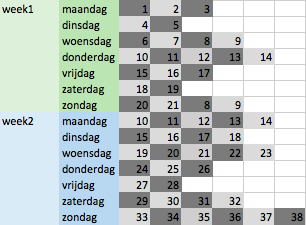
\includegraphics{dataset.png}
	\caption[visuele voorstelling dataset]{visuele voorstelling van een dataset van 2 weken met 38 reservaties}
\end{figure}
\section{Eenvoudige toewijzing}
Voor elke reservatie in de dataset zal geprobeerd worden een beschikbare auto toe te wijzen. Met de implementatie van de eenvoudige toewijzing wordt getracht het huidige reservatiemechanisme te modelleren. De volgorde dat de reservaties in de dataset zitten is de volgorde waarmee de reservaties toekomen bij het systeem. De eenvoudige toewijzing is ook weergegeven in het diagram in figuur 3.2. Alle reservaties in de dataset worden overlopen startend met de eerste reservatie op week1 maandag en eindigend, in dit onderzoek, bij week4 op zondag. De daglijst van reservaties wordt overlopen in de volgorde dat de reservaties in de lijst staan. Uit de beschikbare auto's wordt telkens een willekeurige auto gekozen tot een auto gevonden wordt die nog niet eerder bekeken werd voor deze reservatie. Indien de auto deze reservatie kan vervullen wordt de auto toegewezen aan de reservatie, indien deze auto reeds bezet is tijdens het tijdsinterval van de reservatie wordt er opnieuw een willekeurige auto gekozen die nog niet eerder geprobeerd werd. Indien alle auto's geprobeerd zijn, maar er was geen toewijzing mogelijk kan deze reservatie niet doorgaan en wordt deze toegevoegd aan de lijst van niet-geserveerde reservaties. Dit proces wordt herhaald voor alle reservaties. Elke succesvolle toewijzing wordt ook opgeslagen. Nadat alle reservaties overlopen zijn kan het service level berekent worden door het aantal reservaties dat kon doorgaan te delen door het totaal aantal reservaties in de dataset. 
\section{Toewijzing met behulp van een CSP}
Voor elke reservatie in de dataset zal opnieuw geprobeerd worden een beschikbare auto toe te wijzen, maar deze keer zal voor elke dag in de dataset een Constraint Satisfaction Problem opgesteld worden en zal getracht worden dit probleem op te lossen (zie ook stand van zaken). Het toewijzen met behulp van een CSP is ook weergegeven in het diagram in figuur 3.3. Met deze aanpak wordt er vanuit gegaan dat alle reservaties voor een bepaalde dag gekend zijn voor aanvang van de eerste reservatie. De toegewezen auto voor een reservatie kan dus nog wijzigen naarmate het CSP opgelost wordt. Alle reservaties worden opnieuw overlopen startend bij week1 maandag en eindigend bij week4 zondag. De daglijst van reservaties wordt overlopen in de volgorde dat de reservaties in de lijst staan. Eén voor één worden de reservaties toegevoegd aan het CSP. Na elke toevoeging wordt het CSP opnieuw opgelost. Indien er door het toevoegen van een reservatie geen consistente oplossing meer gevonden kan worden, met andere woorden niet elke reservatie kreeg een auto toegewezen, wordt de reservatie terug verwijderd uit het probleem en toegevoegd aan de lijst van niet-geserveerde reservaties. Dit proces wordt herhaald voor elke reservatie van die dag. De uiteindelijke toewijzing voor die dag wordt ook opgeslagen om de tijd dat de auto's actief waren te kunnen berekenen. Voor elke dag in de dataset wordt gestart met een nieuw, leeg CSP. Nadat alle dagen overlopen zijn kan het service leven berekent worden door het aantal reservaties dat kon doorgaan te delen door het totaal aantal reservaties in de dataset. Voor het oplossen van het CSP wordt gebruik gemaakt van een externe softwarebibliotheek.





